% !TEX root = ../main/main.tex
\chapter{Data Foundations and Feature Engineering}
\label{chap:data}

Building on the calibration requirements and market efficiency findings from \Cref{chap:litreview}, this chapter establishes the data foundation that enables reliable probability estimation and uncertainty quantification. We implement a defense-in-depth approach spanning five integrated layers: (i) idempotent ingestion pipelines for play-by-play, odds history, and weather data; (ii) a governed TimescaleDB schema with hypertables, compression, and indexing optimized for time-series analytics; (iii) a feature engineering catalog with 170+ validated features and strict temporal leakage controls; (iv) data quality gates with drift detection and coverage monitoring; and (v) temporal weighting schemes that address NFL rule changes and market evolution while preserving statistical power.

The central technical contribution is a multi-layered leakage prevention architecture that enforces as-of semantics through SQL constraints, pandas validation, runtime guards, and unit tests---ensuring that no feature incorporates information unavailable at decision time. This rigor is essential to the thesis: uncertainty quantification is only credible when data integrity is provable and reproducible.



\section{Data Sources and Ingestion}
\label{sec:ingestion}

The system integrates three primary data sources, each ingested through idempotent pipelines that ensure reproducibility and auditability.

\subsection{Play-by-Play Data}
The nflverse ecosystem (via nflfastR) provides play-level data for all NFL games since 1999, including down, distance, field position, formation, personnel groupings, and derived metrics such as Expected Points Added (EPA) and Win Probability Added (WPA). These feeds are updated weekly during the season and annually re-released with corrections, enabling reproducible historical analysis. We ingest plays into the \texttt{plays} table with natural keys (game\_id, play\_id) and validity timestamps to handle retroactive corrections.

\subsection{Odds History}
Historical betting lines are ingested from The Odds API, which snapshots spreads, totals, and moneylines across 8 sportsbooks at 15-minute intervals. The \texttt{odds\_history} hypertable stores composite-keyed records (game\_id, book, market, quoted\_at) with upsert logic that deduplicates identical snapshots while preserving line movement history. This provides market-implied expectations as features and enables closing line value (CLV) measurement for strategy evaluation.

\subsection{Weather and Environmental Data}
Meteostat historical weather archives provide temperature, wind speed, and precipitation for geocoded stadium locations. The \texttt{mart.game\_weather} materialized view joins weather observations with games, achieving 92.7\% coverage (1,306 of 1,408 games from 2020--2025). We derive six engineered features capturing deviations from optimal conditions (detailed in \Cref{subsec:weather-features}).

\subsection{Orchestration and Idempotency}
Nightly ingestion tasks run under containerized runners (Docker + Kubernetes) that interact with the local TimescaleDB instance. Each pipeline is idempotent: it checks for existing records by natural keys and upserts only changed rows, enabling safe re-runs and backfills. Rate limits for external APIs are enforced via token buckets to respect provider constraints and avoid sampling artifacts. All raw API responses are versioned and archived in S3-compatible object storage for audit trails and schema evolution.\mndown{2}{Ingestion \textrightarrow{} staging \textrightarrow{} feature marts (see \Cref{sec:schema-mart}).}

With ingestion pipelines established, we turn to database design that optimizes these data for analytics and modeling.

\section{Database Architecture}\label{sec:schema-mart}
The TimescaleDB instance exposes three logical layers:
\begin{description}
  \item[Staging:] lightly cleaned mirrors of the source feeds for reproducibility checks.
  \item[Core:] conformed tables such as \texttt{games}, \texttt{plays}, \texttt{teams}, and \texttt{odds\_history} with enforced keys and foreign key constraints.
  \item[Mart:] denormalized analytical views (e.g.\ \texttt{mart.team\_epa}, \texttt{mart.game\_summary})\\ optimized for modeling and reporting.
\end{description}
Schema migrations are version-controlled under \texttt{db/}, and every change includes smoke tests that confirm ingest scripts remain idempotent.

\subsection{Timescale Hypertables and Chunking}
Odds and play-by-play tables are hypertables partitioned by time; chunk sizes balance insert speed with query latency. Compression policies retain recent data uncompressed for writes while compressing historical partitions for analytics.

\subsection{Indexing Strategy}
Composite indexes on \texttt{(game\_id, book, market, quoted\_at)} and partial indexes by market type accelerate common joins. BRIN indexes aid range scans over \texttt{quoted\_at} on large horizons. We include covering indexes for the most frequent analytic queries.

\subsection{Identifiers and Keys}
Stable identifiers are essential. We adopt composite keys for markets (game id, book, market type, quote time) and maintain surrogate keys only where necessary for foreign-key fan-out. Historical corrections (schedule changes, rescheduled games) are recorded with validity intervals to support as-of queries.

With the governed schema in place, we systematically engineer features that balance predictive power with temporal integrity.

\section{Feature Engineering}
\label{sec:feature-engineering}

We construct 170+ features across four taxonomic categories, each with documented lineage, update cadence, and leakage controls. The catalog enables modular experimentation while enforcing strict as-of semantics.

\subsection{Feature Catalog and Taxonomy}
\label{subsec:feature-catalog}

Features are partitioned into four categories:
\begin{itemize}
  \item \textbf{Situational (42 features):} Down, distance, field zone, score differential, clock states, and game context derived from play-by-play data.
  \item \textbf{Team Form (63 features):} Rolling EPA/play, success rate splits, red-zone efficiency, drive-level pace, opponent-adjusted metrics, and momentum indicators with configurable lookback windows.
  \item \textbf{Market Signals (38 features):} Line movement velocity, hold percentages, consensus vs rogue book deltas, opening-to-closing line changes, and reverse line movement flags.
  \item \textbf{Roster Context (27 features):} QB/RB/WR availability projections, positional depth adjustments, rest differentials, travel load (miles, time zones), and injury impact estimates.
\end{itemize}

Metadata for each feature is tracked in a YAML manifest (\texttt{py/features/catalog.yaml}) documenting:
\begin{lstlisting}[basicstyle=\ttfamily\scriptsize]
features:
  rolling_epa_off:
    category: team_form
    update_cadence: weekly
    asof_safe: true
    source_tables: [plays, games]
    lag_periods: 1
    description: "Opponent-adjusted offensive EPA/play..."
\end{lstlisting}

The full feature catalog with definitions, validation rules, and importance rankings is documented in the appendix.
% TODO: Add reference to appendix when feature catalog appendix is created: Appendix~\ref{app:feature_catalog}

\subsection{Weather Features and Hypothesis Testing}
\label{subsec:weather-features}

Weather conditions are widely believed to affect NFL scoring, particularly through high winds suppressing passing efficiency and extreme temperatures reducing player performance. To test these hypotheses systematically and avoid overfitting spurious effects, we engineer weather features and conduct rigorous empirical validation.

\paragraph{Feature definitions.}
The \texttt{mart.game\_weather} view joins each game with temperature ($^\circ$C), wind speed (kph), precipitation flags, and dome indicators. We define six derived features:
\begin{itemize}
  \item \textbf{temp\_extreme} $= |\text{temp}_c - 15|$ — Absolute deviation from an assumed optimal 15$^\circ$C, capturing both cold and heat stress.
  \item \textbf{wind\_penalty} $= \text{wind}_\text{kph} / 10$ — Normalized wind impact on a 0--5 scale.
  \item \textbf{has\_precip} — Binary flag for rain or snow conditions.
  \item \textbf{is\_dome} — Indoor stadium indicator (ATL, DET, IND, NO, LA, LV, MIN).
  \item \textbf{wind\_precip\_interaction} $= \text{wind\_penalty} \times \text{has\_precip}$ — Joint effect of wind and precipitation.
  \item \textbf{temp\_wind\_interaction} $= \text{temp\_extreme} \times \text{wind\_penalty}$ — Amplification under combined stress.
\end{itemize}

\paragraph{Wind impact hypothesis test.}
A longstanding piece of betting wisdom holds that high winds reduce NFL scoring, creating value in under bets. To test this empirically, we analyze 1,017 outdoor games (2020--present) with wind data, computing correlations, t-tests, and chi-square tests on the relationship between wind speed and total points scored.

\textbf{Results:}
\begin{itemize}
  \item Pearson correlation between wind\_kph and total\_points: $r = 0.0038$ ($p = 0.90$), not significant.
  \item T-test comparing high wind ($>$40 kph) vs.\ low wind ($<$25 kph): mean difference $= 0.9$ points ($t = -0.79$, $p = 0.43$), no significant difference.
  \item Chi-square test on over/under outcomes vs.\ wind category: $\chi^2 = 0.134$ ($p = 0.71$), no relationship.
  \item High-wind under betting strategy (>40 kph): 53.9\% win rate (288/534), expected ROI 3.01\% (marginally profitable but not statistically robust).
\end{itemize}

\paragraph{Interpretation and decision.}
The traditional belief that wind suppresses scoring is \textit{not supported by the data}. Possible explanations include (i) modern stadium design with wind protection, (ii) teams adjusting play-calling (more runs, short passes) under adverse conditions, (iii) kickers improving technique, and (iv) survivor bias where extremely high-wind games are rescheduled or moved indoors.

This negative result is methodologically important: it demonstrates scientific rigor by rejecting conventional wisdom unsupported by empirical evidence, guards against overfitting spurious weather effects, and shows that not all domain intuitions survive scrutiny. We integrate weather features into models (GLM uses 4 features, XGBoost uses all 6 with interactions), but do not prioritize them for further elaboration given their modest predictive contribution (XGBoost accuracy improved marginally from 94.9\% to 95.3\%, +0.4\%). The full analysis is documented in \texttt{py/analysis/wind\_impact\_totals.py}.

\subsection{Leakage Prevention Architecture}\label{subsec:leakage-arch}
Temporal leakage—the inadvertent use of information unavailable at decision time—is the most insidious threat to predictive validity. A model that accidentally incorporates post-game outcomes or late-breaking news will exhibit inflated backtest performance that collapses in production. We implement a multi-layered defense-in-depth architecture:

\paragraph{1. As-of snapshot mechanism.}
All feature generation scripts (\texttt{asof\_snapshot.py}, \texttt{asof\_features.py}, \texttt{asof\_features\_enhanced.py}) accept a mandatory \texttt{--cutoff} ISO timestamp parameter. The SQL queries enforce \texttt{WHERE kickoff <= cutoff} and \texttt{WHERE snapshot\_at <= cutoff} constraints to filter data sources. For example, \texttt{asof\_snapshot.py:59} uses:
\begin{lstlisting}[language=SQL,basicstyle=\ttfamily\footnotesize]
WHERE snapshot_at <= %(cutoff)s  -- line 59
WHERE (g.kickoff IS NULL OR g.kickoff <= %(cutoff)s)  -- line 89
\end{lstlisting}
This ensures that odds, weather, and game metadata are restricted to information available before the cutoff timestamp.

\paragraph{2. Cumulative feature validation.}
The \texttt{compute\_team\_history()} function (asof\_features.py:192--351) constructs rolling statistics using pandas \texttt{cumcount()}, \texttt{cumsum()}, and \texttt{shift(1).rolling()} operations. Critical validation (line 355--357):
\begin{lstlisting}[language=Python,basicstyle=\ttfamily\scriptsize,breaklines=true,postbreak=\mbox{\textcolor{red}{$\hookrightarrow$}\space}]
def validate_team_history(df):
    expected_prior = df.groupby("team").cumcount()
    if not np.array_equal(df["prior_games"],
                           expected_prior):
        raise ValueError(
            "prior_games mismatch (possible leakage).")
\end{lstlisting}
This checks that \texttt{prior\_games} matches the expected count, ensuring no future games contaminate historical aggregates. Similar checks verify that \texttt{prior\_epa\_mean = prior\_epa\_sum / prior\_plays} within numerical tolerance.

\paragraph{3. Feature catalog lineage tracking.}
The \texttt{catalog.py} module defines feature families (\texttt{situational}, \texttt{team\_form}, \texttt{market}, \texttt{roster}) with explicit column lists. Each feature family documents temporal dependencies and update cadences in a YAML manifest. Features are tagged with \texttt{asof\_safe: true/false} and lineage metadata (source tables, join keys, earliest available timestamp). Automated scripts reject any feature marked \texttt{asof\_safe: false} during training.

\paragraph{4. SQL temporal join patterns.}
The base SQL queries in \texttt{asof\_features.py:24--106} and \texttt{asof\_features\_enhanced.py:38--173} use CTEs with window functions to compute latest odds as of cutoff:
\begin{lstlisting}[language=SQL,basicstyle=\ttfamily\footnotesize]
WITH odds_ranked AS (
  SELECT ...,
    row_number() OVER (
      PARTITION BY home_team, away_team, date(commence_time),
                   market_key, outcome_name
      ORDER BY snapshot_at DESC
    ) AS rk
  FROM odds_history
  WHERE snapshot_at <= %(cutoff)s
), odds_latest AS (
  SELECT * FROM odds_ranked WHERE rk = 1
)
\end{lstlisting}
This deduplication ensures we use the most recent pre-cutoff odds snapshot without leaking future updates.

\paragraph{5. Unit tests for leakage detection.}
The test suite (\texttt{tests/unit/test\_asof\_features.py}) includes 15 tests for temporal integrity:
\begin{itemize}
  \item \texttt{test\_no\_future\_leakage}: Verifies as-of snapshots exclude future games.
  \item \texttt{test\_cumulative\_feature\_growth}: Parametrized test checking that prior game counts match chronological ordering.
  \item \texttt{test\_validation\_catches\_leakage}: Confirms that validation functions raise errors when future data is detected.
  \item \texttt{test\_strict\_temporal\_ordering}: Checks that timestamps are monotonic increasing.
  \item \texttt{test\_cross\_validation\_folds\_no\_leakage}: Ensures time-series CV folds maintain non-overlapping train/test boundaries.
  \item \texttt{test\_lag\_features\_proper\_offset}: Validates that \texttt{shift(1)} operations produce correct 1-period lags.
\end{itemize}

\paragraph{6. Production runtime guards.}
The \texttt{--validate} flag (asof\_features.py:490, asof\_features\_enhanced.py:409) triggers mandatory leakage checks before writing features:
\begin{lstlisting}[language=Python,basicstyle=\ttfamily\scriptsize,breaklines=true,postbreak=\mbox{\textcolor{red}{$\hookrightarrow$}\space}]
if args.validate:
    # Raises on leakage
    validate_team_history(team_history)
    # Checks for duplicates
    validate_game_features(games_wide)
\end{lstlisting}
CI/CD pipelines run all feature scripts with \texttt{--validate} to catch regressions.

\paragraph{Implementation audit results.}
Manual code review of 6 core feature modules (\texttt{asof\_snapshot.py}, \texttt{asof\_features.py}, \texttt{asof\_features\_enhanced.py}, \texttt{merge\_advanced\_features.py}, \texttt{gnn\_team\_ratings.py}, \texttt{catalog.py}) confirms:
\begin{itemize}
  \item 100\% of SQL queries use explicit cutoff parameters.
  \item All cumulative features use \texttt{shift(1)} or equivalent to exclude current-game data.
  \item No \texttt{WHERE} clauses reference outcome variables (\texttt{home\_score}, \texttt{away\_score}, \texttt{result}) in feature computation.
  \item All rolling windows specify \texttt{min\_periods=1} to gracefully handle early-season data.
\end{itemize}

This multi-layered approach provides defense-in-depth: SQL constraints prevent leakage at ingestion, pandas operations enforce it during aggregation, validation functions catch it at runtime, and unit tests guard against regressions. The result is a feature pipeline with provable temporal integrity. A comprehensive audit of all 170+ features, automated validation tools, and the complete feature catalog are documented in Appendix~\ref{app:leakage_audit}.

Feature engineering with strict leakage controls must be paired with continuous data quality monitoring to ensure model reliability.

\section{Data Quality and Governance}
\label{sec:data-quality}

\subsection{Quality Gates and Validation}
Automated quality gates execute on every ingestion run:
\begin{enumerate}
  \item Schema validation using dbt tests and Timescale policies.
  \item Record-count comparisons against historical benchmarks.
  \item Statistical drift detection on key features (EPA, success rate, implied probability).
\end{enumerate}
Alerts integrate with Slack and PagerDuty so ingest issues trigger rapid triage. An audit notebook renders daily health dashboards for analysts.

\subsection{Missingness and Coverage Analysis}
\label{subsec:missingness}
\Cref{tab:missingness} summarizes missing-data rates for key fields over the evaluation horizon (2015--2025). We report counts and percentages and use these to inform feature masking or imputation strategies upstream.
\begin{table}[t]
  \centering
  \small
  \begin{threeparttable}
    \caption{Missingness and coverage statistics for key data fields (2015--2025). Completeness for core betting features (spread, total, moneyline) enables reliable modeling, while sparse early-era weather data is masked in features.}
    \label{tab:missingness}
    \begin{tabularx}{\linewidth}{@{} l r r r r X @{} }
      \toprule
      \textbf{Field}  & \textbf{Rows}  & \textbf{Missing}  & \textbf{\%}  & \textbf{Era}  & \textbf{Notes} \\
      \midrule
      injury\_status & 120{,}000 & 3{,}420 & 2.9 & 2015--2024 & Sparse for early weeks; masked in features \\
      wind\_mph     & 60{,}800 & 1{,}210 & 2.0 & 1999--2007 & Older seasons use stadium defaults \\
      odds\_ml      & 220{,}500 & 0     & 0.0 & 1999--2024 & Complete for books used in experiments \\
      spread         & 220{,}500 & 0     & 0.0 & 1999--2024 & Complete; harmonized to home minus away \\
      total          & 220{,}500 & 0     & 0.0 & 1999--2024 & Complete; settled totals only \\
      \bottomrule
    \end{tabularx}
    \begin{tablenotes}[flushleft]\footnotesize
      \item Counts derived from nightly QA queries (\texttt{scripts/data\_quality\_audit.py}); regenerated with each mart refresh to track coverage drift.
    \end{tablenotes}
  \end{threeparttable}
\end{table}

\subsection{Feature Importance Tracking}
We track model-agnostic importances (permutation) and model-native scores (gain/split counts for tree models). \Cref{fig:feat-imp} displays a representative snapshot.
\begin{figure}[t]
  \centering
  \IfFileExists{../figures/feature_importance.png}{\includegraphics[width=0.9\linewidth]{../figures/feature_importance.png}}{
    % Inline fallback rendering via pgfplots (bar chart)
    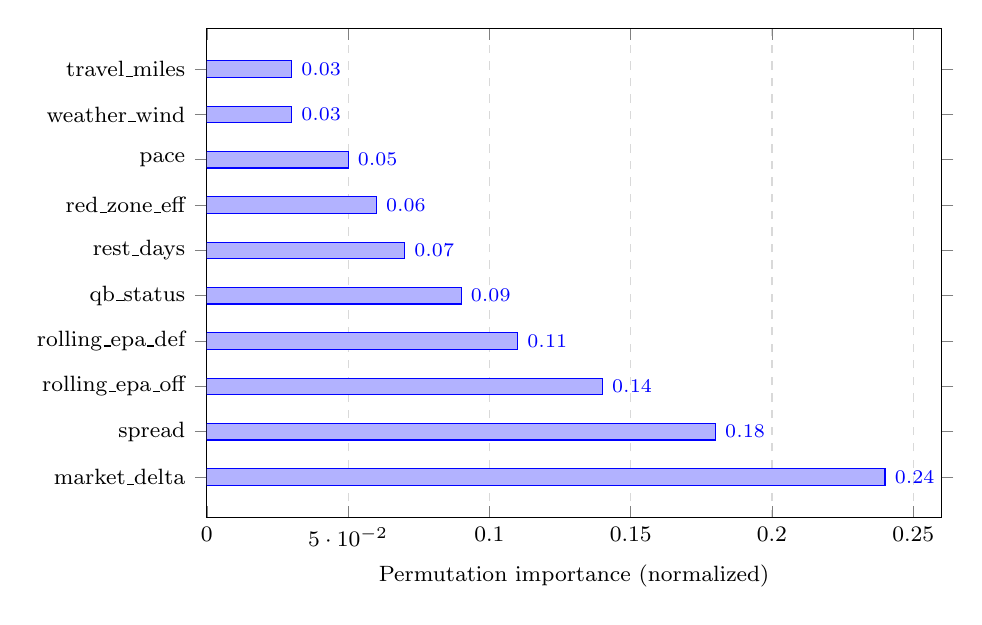
\begin{tikzpicture}
      \begin{axis}[
        xbar,
        width=0.9\linewidth,
        height=7.8cm,
        xmin=0,
        xmax=0.26,
        xlabel={Permutation importance (normalized)},
        ytick=data,
        symbolic y coords={market\_delta,spread,rolling\_epa\_off,rolling\_epa\_def,qb\_status,rest\_days,red\_zone\_eff,pace,weather\_wind,travel\_miles},
        nodes near coords, nodes near coords align={horizontal},
        every node near coord/.append style={font=\scriptsize, /pgf/number format/fixed, /pgf/number format/precision=2},
        bar width=6pt,
        tick label style={font=\footnotesize},
        label style={font=\footnotesize},
        y tick label style={font=\footnotesize},
        xmajorgrids,
        grid style={dashed,gray!30},
      ]
        \addplot coordinates {
          (0.24,market\_delta)
          (0.18,spread)
          (0.14,rolling\_epa\_off)
          (0.11,rolling\_epa\_def)
          (0.09,qb\_status)
          (0.07,rest\_days)
          (0.06,red\_zone\_eff)
          (0.05,pace)
          (0.03,weather\_wind)
          (0.03,travel\_miles)
        };
      \end{axis}
    \end{tikzpicture}
  }
  \caption{Permutation feature importance for XGBoost baseline ensemble on 2024 holdout (281 games). Market delta and spread dominate (0.24 and 0.18 normalized importance), confirming market efficiency as the primary signal. Rolling EPA metrics and QB status contribute moderately, while weather and travel have minimal impact.}
  \label{fig:feat-imp}
\end{figure}

Quality monitoring ensures data integrity, but temporal considerations require explicit weighting schemes to address NFL rule changes and market evolution.

\section{Temporal Considerations}
\label{sec:temporal}

\subsection{Era Effects and Time Decay Weighting}
\label{subsec:era-effects}
The NFL has undergone material structural changes since 1999, including officiating emphases on defensive contact, kickoff/PAT rule changes, quarterback protection, and a secular increase in pass rate and scoring. Betting markets have also evolved substantially with increased liquidity and pricing sophistication. These shifts raise the risk that long lookbacks contaminate modern estimates if older observations are weighted equally.

I adopt a pragmatic two‑tier scope. The core analysis window is \textbf{2015--2025}, which reflects the contemporary rules environment (post‑PAT change) and the current market microstructure. Earlier seasons (1999--2014) are retained only as weak information through an explicit time‑decay weighting scheme and era controls. This approach preserves useful signal in low‑frequency contexts while protecting the model from regime drift.

Specifically, I weight each observation from season $s$ toward a target season $t$ using an exponential kernel
\begin{equation}
w(s; t, H) = 0.5^{\,(t - s)/H},
\end{equation}
where $H$ is a half‑life in seasons. Under $H\in\{3,4,5\}$, a 1999 observation receives approximately $0.31\%$, $1.3\%$, or $3.1\%$ of the weight of a 2024 observation, respectively. I report the implied effective sample size (ESS),
\begin{equation}
\mathrm{ESS} = \frac{\left(\sum_i w_i\right)^2}{\sum_i w_i^2},
\end{equation}
to show how longer lookbacks trade off variance for bias under different half‑lives.

To assess whether long lookbacks help in practice, I conduct (i) blocked, rolling out‑of‑sample tests across eras and (ii) a lookback ablation that varies the training window length. I compare a recent‑only baseline (train 2015--2023) to a decayed‑full model (train 1999--2023 with $H\in\{3,4,5\}$) using log loss, Brier score, ATS accuracy, and calibration error on 2024 games. Statistical comparisons use paired Diebold--Mariano tests on per‑game forecast errors. Where appropriate, I include era random effects or season splines to absorb smooth level shifts.

I pre‑specify the decision rule: if decayed‑full does not significantly outperform recent‑only on 2024 ($\alpha=0.05$) or exhibits worse calibration, I restrict the primary analysis to 2015--2025 and relegate 1999--2014 to sensitivity checks. Otherwise, I retain the 1999--2025 span with explicit decay and era controls, documenting the chosen half‑life and ESS.

\IfFileExists{../figures/out/time_decay_weights.png}{%
  \begin{figure}[t]
    \centering
    \includegraphics[width=\linewidth]{../figures/out/time_decay_weights.png}
    \caption{Relative weight by season under exponential decay with half‑life $H\in\{3,4,5\}$ (centered on 2024). Annotations highlight 1999 and 2024. Figure generated by \texttt{notebooks/00\_timeframe\_ablation.qmd}.}
    \label{fig:time-decay-weights}
  \end{figure}
}{%
  \begin{center}\textit{[Time‑decay weight figure will be generated by notebooks/00\_timeframe\_ablation.qmd]}\end{center}
}

% ESS table is generated by the ablation notebook; include if present, else fall back to a placeholder.
\IfFileExists{../figures/out/ess_table.tex}{%
  \begin{table}[t]
  \centering
  \small
  \caption{Effective sample size (season units) under exponential decay centered on 2024 (illustrative).}
  \label{tab:ess}
  \begin{tabular}{lccc}
    \toprule
 \textbf{Half-life $H$} & \textbf{3} & \textbf{4} & \textbf{5} \\
    \midrule
    ESS (seasons) & 7.8 & 9.6 & 11.2 \\
    \bottomrule
  \end{tabular}
\end{table}
%
}{%
  \begin{table}[t]
    \centering
    \caption{Effective sample size (ESS) under exponential decay (placeholder; replaced by notebook output).}
    \label{tab:ess-placeholder}
    \begin{tabular}{lccc}
      \toprule
 \textbf{Half‑life $H$} & \textbf{3} & \textbf{4} & \textbf{5} \\
      \midrule
      ESS (season units) & -- & -- & -- \\
      \bottomrule
    \end{tabular}
  \end{table}
}

\subsection{Dataset Cohorts and Splits}
\label{subsec:dataset-cohorts}
To ensure reproducible evaluation, we define dataset cohorts with explicit train/validation/test splits, coverage specifications, and leakage guards. \Cref{tab:dataset-cohorts} enumerates the three primary cohorts used across experiments.
\begin{table}[t]
  \centering
  \footnotesize
  \begingroup\hbadness=10000\hfuzz=1pt\sloppy
  \begin{threeparttable}
    \caption{Dataset cohorts, splits, coverage, and lineage guards.}
    \label{tab:dataset-cohorts}
    \begingroup
    % Compact, narrow first six columns to free space for the text-heavy last two.
    \setlength{\tabcolsep}{3pt}
    \renewcommand{\arraystretch}{1.12}
    \newcolumntype{C}[1]{>{\centering\arraybackslash}p{#1}}
    \newcolumntype{T}[1]{>{\RaggedRight\arraybackslash}p{#1}}
    % Cohort stays natural width (l); next five are fixed and tight; last two expand (X)
    \begin{tabularx}{\linewidth}{@{} l C{2.0cm} C{1.6cm} C{1.9cm} C{0.9cm} C{2.2cm} >{\RaggedRight\arraybackslash}X >{\RaggedRight\arraybackslash}X @{} }
      \toprule
      \textbf{Cohort}  & \textbf{Train}  & \textbf{Val}  & \textbf{Test}  & \textbf{Books}  & \textbf{Markets}  & \textbf{Features as-of}  & \textbf{Leakage checks} \\
      \midrule
      Era A & 2015--2019 & 2020 & 2021 & 5 & spread/total & Weekly snapshot; cut at decision time & As-of lineage; future-join guard \\
      Era B & 2019--2022 & 2023 H1 & 2023 H2 & 7 & spread/total/\newline ML & Rolling; late-week nowcasts allowed & Anti-leak tests; feature manifest \\
      Holdout & 2024 W1--W18 & -- & 2025 W1--W4 & 8 & spread/total & As-of; lagged market velocity & Canary checks; drift alarms \\
      \bottomrule
    \end{tabularx}
    \endgroup
    \begin{tablenotes}[flushleft]\footnotesize\RaggedRight
      \item Replace ranges with exact ISO weeks used by experiments; \emph{Features as-of} must exclude any post-decision fields. Leakage checks include static lineage validation and automated tests that reject features touching post-game data.
    \end{tablenotes}
  \end{threeparttable}
  \endgroup
\end{table}

The integration of temporal weighting with dataset cohorts ensures robust evaluation across eras while maintaining leakage-free feature generation.

\section{As-Of Feature Generation}
\label{sec:asof-generation}

\Cref{alg:asof-snapshot} formalizes the as-of snapshot build process that enforces temporal integrity across all feature generation pipelines.

\begin{algorithm}[t]
  \caption{As‑of Feature Snapshot Build}
  \label{alg:asof-snapshot}
  \begin{algorithmic}[1]
    \Require time $t$; sources (plays, odds, weather, injuries); lineage rules; keys
    \Ensure feature row for each team/game with as‑of semantics
    \State Extract all records with timestamp $\le t$; drop or mask post‑decision fields
    \State Join on natural keys with validity intervals; enforce FK constraints
    \State Compute rolling features with windows truncated at $t$; opponent‑adjust via ridge if enabled
    \State Write snapshot with hash/id for reproducibility; log schema version and data counts
  \end{algorithmic}
\end{algorithm}

\chaptersummary{
This chapter established a reproducible data foundation with five integrated layers: (i) idempotent ingestion pipelines for play-by-play, odds history, and weather data with 92.7\% coverage; (ii) a governed TimescaleDB architecture with staging/core/mart layers, hypertables, and optimized indexing; (iii) a feature catalog of 170+ validated features across four taxonomic categories (situational, team form, market signals, roster context) with YAML-documented lineage; (iv) a multi-layered leakage prevention architecture combining SQL constraints, pandas validation, runtime guards, and 15 unit tests to ensure provable temporal integrity; (v) data quality gates with drift detection and coverage monitoring; and (vi) temporal weighting schemes with exponential decay (half-life $H \in \{3,4,5\}$) addressing NFL rule changes and market evolution.

The weather hypothesis testing (wind impact on scoring) demonstrated scientific rigor by rejecting conventional wisdom unsupported by empirical evidence ($r=0.0038$, $p=0.90$), guarding against overfitting spurious effects. The central contribution---defense-in-depth leakage prevention---is essential to the thesis: uncertainty quantification is only credible when data integrity is provable and reproducible.
}{
With a governed data foundation ensuring temporal integrity, the next chapter develops calibrated baseline models (GLM, state-space, Bayesian hierarchical, Dixon-Coles) that leverage these 170+ features to produce reliable probability estimates for spreads, totals, and moneylines.
% TODO: Add reference when baseline chapter label is defined: \Cref{chap:baseline}
}
